\documentclass[uplatex]{jsarticle}
\usepackage[top=20truemm, bottom=20truemm, left=20truemm, right=20truemm]{geometry}
\usepackage{url}
\usepackage{booktabs}
\usepackage{here}
\usepackage{amsmath, amssymb}
\usepackage[dvipdfmx]{graphicx}
\usepackage{listings}
\lstset{
    basicstyle = \ttfamily\scriptsize,
}

\renewcommand{\lstlistingname}{ソースコード}

\title{
    \vspace{-1.5cm}
    サイバーセキュリティ Assignment 3 \\
    Incident 2
    \author{Group 6}
}

\begin{document}
\maketitle

\subsubsection*{担当者 SubgroupB}
\begin{table}[H]
    \begin{tabular}{|c|l|l|}
        \hline
        学生番号 & 氏名 & 所属研究室\\
        \hline\hline
        2011156 & 成 泰鏞 & ソフトウェア工学研究室\\
        \hline
        2011231 & 久田 祥平 & ソーシャルコンピューティング研究室\\
        \hline
        2011271 & 森本 康太 & 情報セキュリティ工学研究室\\
        \hline
    \end{tabular}
\end{table}

\section*{Step 1}
\subsection*{Question}
For each incident, provide a detailed summary of the incident report toward cybersecurity professionals, by fully mobilizing concepts that you learned through these lectures. Create a timeline of the incident, as well as a fishbone diagram, that illustrates root cause and other important events in order to help with the understanding.
\subsection*{Answer}
我々は,2017年2月に発生したWebコンテンツ管理システム WordPress を利用する
Webページが改ざんされるインシデントについて調査した.
世界中で150万以上のWebページが改造され,
国内でも行政や議員のWebサイトが改ざん被害を受けた.
改ざんの被害自体はいたずらのような改変のみで,
フィッシングサイトやコンテンツにマルウェアを仕込むような改変は報告されておらず,
個人情報の流出といった深刻なものはなかった.
しかしながら,病院や当時の五輪相といった公的な情報を提供するホームページも改ざんされた
\footnote{
    サイト改ざん相次ぐ 病院や大学,五輪相も被害: 日本経済新
    : \url{https://r.nikkei.com/article/DGXLASDG06HFY_W7A200C1CC1000?s=5}
}
ことから,
影響は小さくないと言える.
WordPress の脆弱性が原因となって引き起こされたインシデントレポートも報告されている.
日本小児循環器学会のインシデントレポート
\footnote{\url{http://jspccs.jp/wp-content/uploads/140206.pdf}}
によると,
ホームページのタイトルが改ざんなどの被害が報告されている.
この脆弱性に対して,
Webコンテンツセキュリティ会社,Sucuri社がWordPressのチームに脆弱性を通知した.
1週間後のアップデートによって,該当する脆弱性は修正された.
WordPress は,脆弱性の内容を公開しないことで被害を最小限にしようと試みた.
しかしながら,脆弱性公開から2日以内に概念実証(以下PoC)方法が,
Web上で共有されたことによって,攻撃手法が広く拡散され,改ざんされる事例は急増した.
また,この改ざんの二次被害としては,
サーチエンジンが改ざんされたページを発見することで,ページランクが下がることが考えられる.
WordPress のこの脆弱性に対して,CVE-2017-1001000
\footnote{
    NVD - CVE-2017-1001000
    : \url{https://nvd.nist.gov/vuln/detail/CVE-2017-1001000}
}
が発行されている.
これによると,機密性や可用性への影響はなく,完全性への影響も限定的ではあるもの,
脆弱性へのアクセスが非常に容易なことよりCVSS3.0スコアは7.5となっている.

\begin{table}[htbp]
    \centering
    \caption{インシデントタイムライン}
    \label{tab:incident_timeline}
    \begin{tabular}{|l|p{12cm}|}
    \hline
    2016年8月16日 & WordPress4.7がリリース,REST APIが追加される \\ \hline
    2016年12月6日 & WordPress4.7がリリース,REST API コンテンツエンドポイントが追加される \\ \hline
    2017年1月11日 & WordPress4.7.1がリリース,4.7から61件のバグが修正される \\ \hline
    2017年1月20日 & Sucuri社がWordpressに脆弱性について警告 \\ \hline
    2017年22~23日 & SucuriやSiteLock,Cloudflare,IncapsulaのようなWebセキュリティー会社が悪意のある攻撃を防ぐFirewallをそのカスタマーに追加 \\ \hline
    2017年26日 & WordPress4.7.2をリリース \\ \hline
    2017年2月1日 & WordPress4.7や4.7.1の脆弱性の内容が公開される. \\ \hline
    2017年2月2日 & 脆弱性に対するPoCがWebページの改ざん方法がオンライン上で共有され,攻撃を試みる事例が多数発生し始める. \\ \hline
    2017年2月6日 & 日本国内における注意喚起が行われる. \\ \hline
    \end{tabular}
\end{table}

\begin{figure}[htbp]
    \centering
    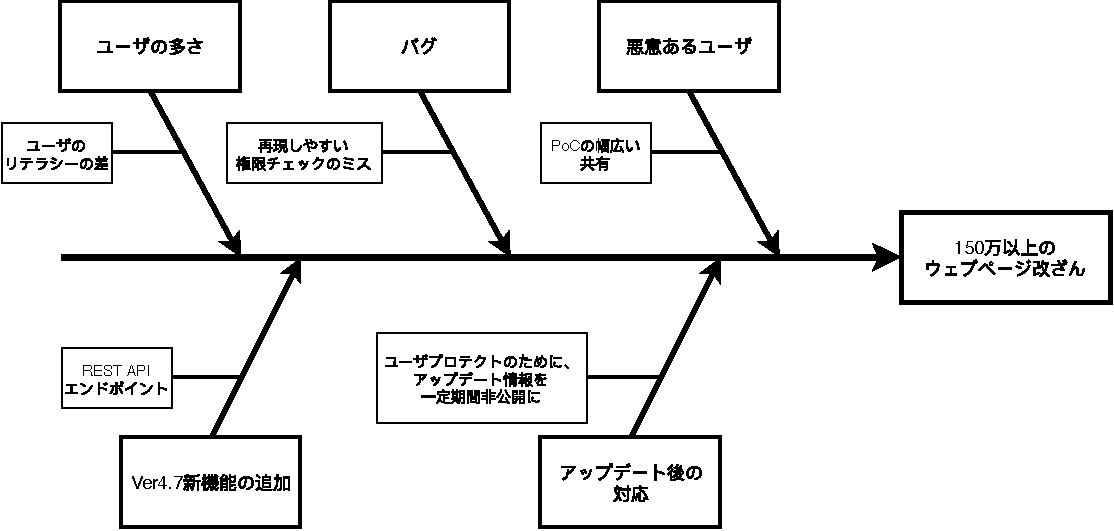
\includegraphics[width=0.8\linewidth]{pic/fishbone-GroupB.pdf}
    \caption{特性要因図}
    \label{fig:fishbone}
\end{figure}

\section*{Step 2}
\subsection*{Question}
Identify technical factors that led to each incident. Based on the real timeline of the particular incident, identify two critical periods where technical intervention was necessary.
\subsection*{Answer}

WordPressの REST API が,インシデントの原因として最大のものであった.
WordPressでは以前からREST APIがプラグインとして用意されていたが,
WordPress 4.7以降で WordPress Coreにバンドルしたことで,
APIで様々な機能が実行できるようになった.今回の脆弱性は,このREST APIにあった.
次に,REST APIのコードを用いて,脆弱性の技術的要因について述べる.
攻撃者は,認証を回避して,id=1のコンテンツの改変を試みたとする.WordPressのREST APIの内部では,以下の2つのメソッドが処理を行う.

\begin{itemize}
    \item \verb|update_item_permissions_check| (権限の確認)
    \item \verb|update_item| (コンテンツの変更)
\end{itemize}

\verb|update_item_permissions_check|メソッド
\footnote{\url{wp-includes/rest-api/endpoints/class-wp-rest-posts-controller.php} (ver4.7.1)}
のソースコード\ref{program1}において,
idに指定されたコンテンツの性質による,メソッドの返り値は表\ref{tab:return_value}の通りである.

\begin{table}[htbp]
    \centering
    \caption{メソッドの返り値}
    \label{tab:return_value}
    \begin{tabular}{|l|l|}
    \hline
    コンテンツの性質 & 返り値 \\ \hline
    存在しないコンテンツ & true \\ \hline
    存在し権限のあるコンテンツ & true \\ \hline
    存在し権限のないコンテンツ & false \\ \hline
    \end{tabular}
\end{table}

\begin{lstlisting}[caption = update\_item\_permissions\_checkメソッド, label = program1]
497:  public function update_item_permissions_check( $request ) {
498:    $post = get_post( $request['id'] );
499:    $post_type = get_post_type_object( $this->post_type );
500:    if ( $post && ! $this->check_update_permission( $post ) ) {
501:      return new WP_Error( 'rest_cannot_edit', __( 'Sorry, you are not allowed to edit this post...
502:    }
503:    if ( ! empty( $request['author'] ) && get_current_user_id() !== $request['author'] &&
                ! current_user_can( $post_type->cap->edit_others_posts ) ) {
504:      return new WP_Error( 'rest_cannot_edit_others', __( 'Sorry, you are not allowed to update ...
505:    }
506:    if ( ! empty( $request['sticky'] ) && ! current_user_can( $post_type->cap->edit_others_posts ) ) {
507:      return new WP_Error( 'rest_cannot_assign_sticky', __( 'Sorry, you are not allowed to make ...
508:    }
509:    if ( ! $this->check_assign_terms_permission( $request ) ) {
510:      return new WP_Error( 'rest_cannot_assign_term', __( 'Sorry, you are not allowed to assign ...
511:    }
512:    return true;
513:  }
\end{lstlisting}

表\ref{tab:return_value}から,存在しないコンテンツが指定された場合,
\verb|update_item_permissions_check| メソッド最後の return文 にて
\verb|true| が返されることになる.
しかし,この「存在しないコンテンツ」については,
ソースコード\ref{program2}の \verb|update_item| メソッドの 526行目にてエラーが返される予定であった.

\begin{lstlisting}[caption=update\_itemメソッド, label=program2]
523:  public function update_item( $request ) {
524:    $id   = (int) $request['id'];
525:    $post = get_post( $id );
526:    if ( empty( $id ) || empty( $post->ID ) || $this->post_type !== $post->post_type ) {
527:      return new WP_Error( 'rest_post_invalid_id', __( 'Invalid post ID.' ), array( 'status' => 404 ) );
528:    }
529:    $post = $this->prepare_item_for_database( $request );
530:    if ( is_wp_error( $post ) ) {
531:      return $post;
532:    }
\end{lstlisting}

ここで,\verb|id=1A| が指定されたときに,\verb|update_item_permissions_check| メソッドと
\verb|update_item| メソッドの両方で呼ばれている \verb|get_post| 関数が
受け取るパラメータを確認すると, \verb|update_item_permissions_check| では,
\verb|get_post('1A')| が呼ばれ,\verb|1A|をIDとするコンテンツはないため,
「コンテンツは存在しない」が返され,チェック結果は \verb|true| となる.
一方,\verb|update_item| メソッドは,\verb|$id| を整数にキャストしているため,
\verb|get_post(1)|が呼ばれ,\verb|ID=1| のコンテンツが変更されることなる.
これにより,本来権限のないコンテンツ \verb|ID=1| に対する更新ができてしまう.
これより,不正なidに対して,REST API内でidの処理に不整合が生じる.
これが今回のインシデントの技術的要因である
\footnote{
    参考
    \url{https://blog.tokumaru.org/2017/02/wordpress-4.7.1-Privilege-Escalation.html}
}
.

次に,技術的に介入が必要とされた時期について述べる.
1つ目の介入点は,Ver4.7のリリース前であると考えられる.
WordPress4.7ではRestAPIコンテンツエンドポイン卜が追加されている.
Ver4.6比較し,Rest APIを通じて以下の機能を編集できるようになっていた.
\begin{enumerate}
    \item 投稿記事(Post) [一覧の取得・表示・追加・更新・削除・revision取得]
    \item 固定ページ(Page) [一覧の取得・表示・追加・更新・削除・revision取得]
    \item メディア [一覧の取得・表示・追加・更新・削除]
    \item コンテントタイプの種類 [表示]
    \item カテゴリー [一覧の取得・表示・追加・更新・削除]
    \item タグ [一覧の取得・表示・追加・更新・削除]
    \item カスタムタクソノミー [表示・編集]
    \item WordPressユーザ [一覧の取得・表示・追加・更新・削除]
    \item コメント [一覧の取得・表示・追加・更新・削除]
\end{enumerate}
これらの機能を維持するために,REST API はデフォルトの状態でONとなっており,これが被害の拡大につながったと考えられる.一般のユーザは,このようなAPIを頻繁に利用するとは考えにくい.それゆえ,デフォルトではREST APIの状態をOFFにするべきであり,必要な場合のみONにするべきであると考えられる.

2つ目の介入点は,4.72のリリース時と考えられる.アップデートから情報公開までに猶予期間を設けたり,Webコンテンツセキュリティ会社を通じてWAFを実装したりと対策はなされていたが,アップデートを強制したり,以前のバージョンの利用を禁止したりと,ユーザーに強制介入できる要素を設けておく必要はあったと考えられる.HP管理者も,セキュリティーアップデートと言う形のVer4.72が公開された時点でアップデートすれば,攻撃が実際に起こるまではタイムラグがあるので,Webページの改ざんを未然に防ぐことはできたと考えられる.

\section*{Step 3}
\subsection*{Question}
Identify human factors that led to each incident. Based on the real situation of the particular incident, describe how best you would deliver risk messages, as an external security consultant, in the two critical periods that you identified in the step 2.
\subsection*{Answer}
インシデントの原因となった人的要因は, 以下の3つが考えられる.
\begin{itemize}
    \item 開発者
    \item 悪意のあるユーザ
    \item WordPress 使用者のHP管理者
\end{itemize}
まず,開発者について述べる.プログラムの傾向として,一部の変数を利用直前にintに変更している.これが潜在的なバグや脆弱性の原因となっていた.入力値について,「数値以外のものをエラーとする」などの変数管理の習慣が必要ではあった.今回はチェックと更新とで異なる入力を用いてたため,両者の不整合がチェック漏れの原因となっている.アプリケーションにおいてAPIは外部との境界線になるため, 入念なチェックが必要である.
次に悪意のあるユーザーについて述べる.悪意のあるユーザーが脆弱性に対するPoCがWebページの改ざん方法がオンライン上で共有を行った. その結果, 他の悪意のあるユーザーが改ざんを行い被害が広がった.
最後にWordPress使用者のHP管理者について述べる.サイトを放置しているHP管理者や仕様変更を拒みアップデートを行わない管理者が多く存在した. 実際, 最新のバージョンを使用しているユーザーは, 42.8\%と半分も存在しない
\footnote{\url{https://ja.wordpress.org/about/stats/}}
. そのためユーザーのリテラシーが低く, 攻撃対象となるサイトが増えてしまい被害が広がった.

次に,リスクメッセージについて,以下の時点で配信するべきと考える.
まず,2016年8月16日: WordPress4.7リリース時点.WordPress開発者に対して, APIのリスクについて伝え,脆弱性のチェックを行うことを推奨する.特に,ver 4.7では REST APIを通じて多くの機能が追加されている.また,過去にもAPIの追加が脆弱性となり,様々なインシデントが発生している点を考慮し,脆弱性のチェックや通常時よりも入念なテストを呼びかけるメッセージが必要であると考える.
次に,2017年1月26日 WordPress4.72のリリース時点.
WordPress使用者に対してアップデートを強く促すメールを配信することを推奨する.
通常,WordPressはアップデートの度に更新通知をメールで配信している.ver 4.72のリリースは,脆弱性を修正する点で,通常より緊急性が高いアップデートであると言える.それゆえ,通常の更新通知ではなく,ユーザに重要度と緊急度高いアップデートであることを強調する必要があったと考える.


\end{document}
